% Open Orders by MSA report builder (macro v2.8): the deck for the 1 hr 30 min team review.
% Three 11 x 17 landscape sheets (ledger, 17 x 11 in) drawn in TikZ, in the house style of open-orders-macro-flow.tex:
%   Sheet 1 "Agenda": a 90-minute timeline. Part 1, current system review (30 min): sheets 2 and 3, 5 min each,
%   then a live build from Lexi's exports (20 min). Part 2, planning for the future (60 min, open): where the data
%   needs to go and the PowerPoint questions (questions 3, 7, 14 to 16 and 18 of open-orders-report-questions.tex).
%   The same Part 2 questions are printed to write on in open-orders-meeting-questions.tex; keep the two in step.
%   Sheet 2 "Design Process": the five steps in the order they were done (map, Copilot, design, generative AI, prove it).
%   Sheet 3: open-orders-macro-flow.tex itself, input with docmute (one source; its title block shows \flowsheet).
% Facts come from the .bas and .py files in this folder, output/.../macro-instructions.md (validation) and
% business-case.md; "10 to 15 prompts on each file" is the owner's own figure.
% Each sheet is laid out on a 12 x 7.5 in grid and scaled by 4/3 to fill the 16 x 10 in drawing area.
% Build: ./build.sh source/open-orders-intake-inventory/open-orders-team-review.tex
\documentclass[10pt]{article}
\usepackage[paperwidth=17in, paperheight=11in, margin=0.5in]{geometry}
\usepackage[T1]{fontenc}
\usepackage{lmodern}
\usepackage{microtype}
\usepackage{enumitem}
\usepackage{xcolor}
\usepackage{tikz}
\usetikzlibrary{positioning, arrows.meta, calc, fit, shapes.geometric, intersections}
\usepackage{docmute}
\usepackage[hidelinks, pdftitle={Open Orders by MSA: Team Review}, pdfauthor={Gust F.}]{hyperref}
\pagestyle{empty}
\setlength{\parindent}{0pt}
\hyphenpenalty=10000
\exhyphenpenalty=10000
\setlist[itemize]{label=\textbullet, leftmargin=0.85em, labelsep=0.35em, itemsep=1.5pt, parsep=0pt,
                  topsep=0pt, partopsep=0pt}
\definecolor{headgreen}{HTML}{548235}
\definecolor{bandgreen}{HTML}{E2EFDA}
\definecolor{flagpeach}{HTML}{FCE4D6}
\tikzset{
  every node/.style={font=\sffamily\small, inner sep=5pt},
  box/.style={draw, line width=0.5pt, fill=white, align=left},
  station/.style={draw, line width=0.5pt, fill=headgreen, text=white, font=\sffamily\bfseries\normalsize,
                  align=center, inner ysep=4pt, text height=1.6ex, text depth=0.45ex},
  flow/.style={-{Stealth[length=9pt, width=6.5pt]}, line width=1.2pt, line join=miter},
  link/.style={-{Stealth[length=6pt, width=4.5pt]}, line width=0.6pt, dash pattern=on 3pt off 2pt},
  note/.style={font=\sffamily\footnotesize, inner sep=2pt},
  % used by sheet 3, the build-flow drawing
  gate/.style={draw, line width=0.8pt, diamond, aspect=2, inner sep=4pt, font=\sffamily\bfseries\small},
  branch/.style={font=\sffamily\bfseries\small, inner sep=3pt},
  % flowchart document symbol: 1.55 x 0.42 in, wavy foot, anchored at its top left corner
  doc/.pic={\draw[line width=0.5pt, fill=white] (0,0) -- (1.55,0) -- (1.55,-0.36)
              .. controls (1.15,-0.5) and (0.45,-0.26) .. (0,-0.42) -- cycle;}
}
\newcommand{\by}[1]{{\footnotesize\itshape #1}\\[3pt]}
\newcommand{\lines}[1]{{\fontsize{7.5}{9}\selectfont #1 lines}}
\newcommand{\peach}[1]{{\setlength{\fboxsep}{1pt}\colorbox{flagpeach}{\textbf{#1}}}}
\newcommand{\badge}[1]{{\setlength{\fboxsep}{2pt}\colorbox{headgreen}{\textcolor{white}{\bfseries #1}}}}
\newcommand{\flowsheet}{3 of 3}
% miniatures of sheets 2 and 3 for the agenda, drawn in each sheet's own 12 x 7.5 coordinates (use in a scaled scope)
\newcommand{\thumbframe}{%
  \draw[line width=0.5pt, fill=white] (0,0) rectangle (12,7.5);
  \fill (0.25,7.0) rectangle (2.6,7.25);}
\newcommand{\thumbdesign}{%
  \thumbframe
  \foreach \a/\b/\c in {0.25/2.74/3.94, 2.98/5.47/4.49, 5.71/9.05/2.76, 9.29/11.73/5.17} {
    \draw[line width=0.3pt] (\a,6.3) rectangle (\b,\c); \fill[headgreen] (\a,6.02) rectangle (\b,6.3);}
  \draw[line width=0.3pt] (0.25,2.62) rectangle (8.59,0.59); \fill[headgreen] (0.25,2.34) rectangle (8.59,2.62);
  \draw[line width=0.3pt] (0.46,2.55) rectangle (2.33,1.97); \draw[line width=0.3pt] (2.98,2.55) rectangle (4.84,1.97);
  \draw[line width=0.3pt] (9.29,2.15) rectangle (11.73,1.1);
  \draw[line width=0.3pt] (5.7,0) -- (5.7,0.42) -- (12,0.42);}
\newcommand{\thumbflow}{%
  \thumbframe
  \foreach \a/\b/\c in {0.26/2.16/3.32, 2.66/4.54/4.93, 5.04/6.9/4.25, 7.4/9.35/3.7, 9.86/11.75/3.64} {
    \draw[line width=0.3pt] (\a,5.8) rectangle (\b,\c); \fill[headgreen] (\a,5.52) rectangle (\b,5.8);}
  \draw[line width=0.3pt] (5.95,4.25) -- (5.95,3.59) (5.42,3.34) -- (5.95,3.59) -- (6.48,3.34) -- (5.95,3.09) -- cycle;
  \draw[line width=0.3pt] (5.95,3.09) -- (5.95,2.55) (4.88,2.55) rectangle (7.02,1.71);
  \draw[line width=0.3pt] (6.48,3.34) -- (7.96,3.34) (2.14,1.6) -| (7.96,3.7);
  \draw[line width=0.3pt] (0.26,2.08) rectangle (2.14,1.12);
  \draw[line width=0.3pt] (10.83,3.64) |- (1.2,0.85) -- (1.2,1.12);
  \draw[line width=0.3pt] (6.91,0) -- (6.91,0.42) -- (12,0.42);}
% title block, one row in the bottom right corner: #1 title, #2 sheet
\newcommand{\titleblock}[2]{%
  \draw[line width=0.5pt] (5.7,0) -- (5.7,0.42) -- (12,0.42);
  \foreach \x in {7.3, 8.95, 9.5, 9.95, 10.75, 11.45} \draw[line width=0.5pt] (\x,0) -- (\x,0.42);
  \foreach \x/\label/\value in {5.7/Title/#1, 7.3/Project/Open Orders by MSA, 8.95/Macro/v2.8, 9.5/Rev./13,
                                9.95/Date/2026-10-15, 10.75/Drawn/Gust F., 11.45/Sheet/#2} {
    \node[anchor=north west, inner sep=0pt, font=\sffamily\fontsize{7}{8}\selectfont] at (\x+0.07,0.36) {\label};
    \node[anchor=south west, inner sep=0pt, font=\sffamily\bfseries\footnotesize] at (\x+0.07,0.07) {\value};
  }}

\begin{document}
% ============================================================================ sheet 1: Agenda
% timeline: 90 minutes from x = 0.5 to x = 11.5 (11/90 in a minute): 0:05 at 1.1111, 0:10 at 1.7222, 0:30 at 4.1667
\noindent
\scalebox{1.333333}{%
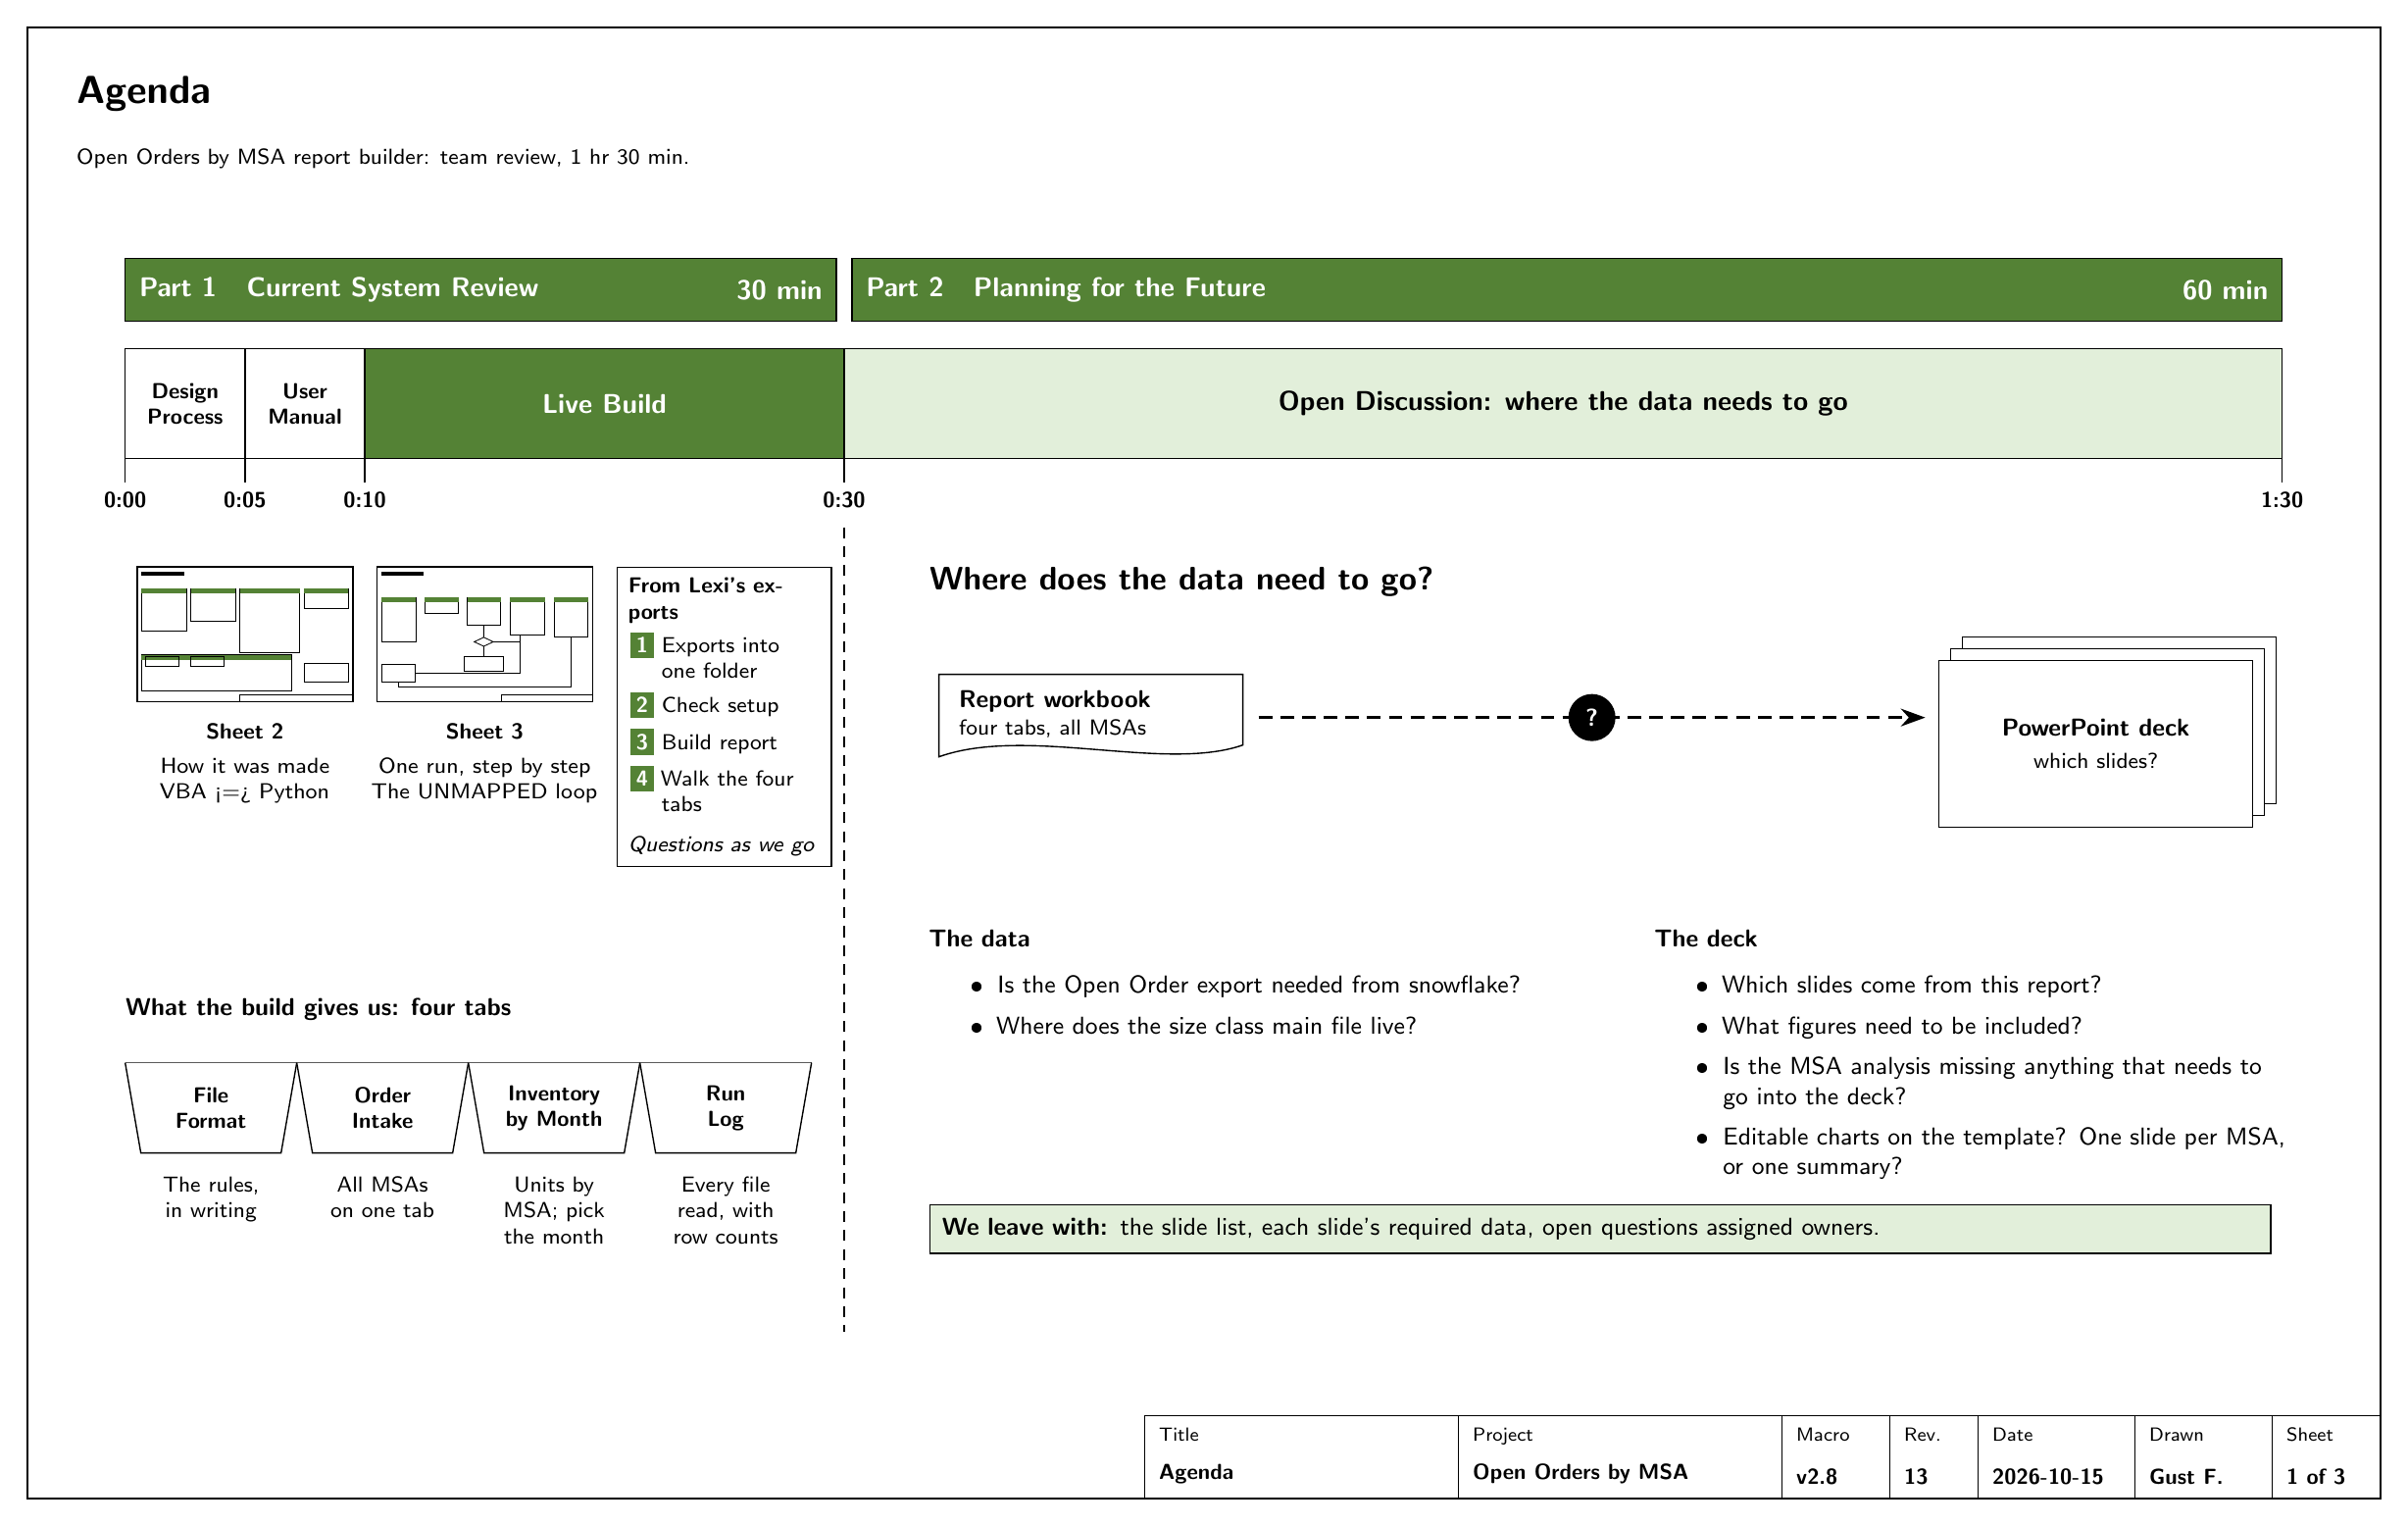
\begin{tikzpicture}[x=1in, y=1in]
\useasboundingbox (0,0) rectangle (12,7.5);
\draw[line width=0.8pt] (0,0) rectangle (12,7.5);

\node[anchor=north west, inner sep=0pt, font=\sffamily\bfseries\fontsize{14}{16}\selectfont]
  at (0.25,7.25) {Agenda};
\node[anchor=north west, inner sep=0pt, font=\sffamily\footnotesize] at (0.25,6.88)
  {Open Orders by MSA report builder: team review, 1 hr 30 min.};


% ---------------------------------------------------------------- the two halves
\draw[line width=0.5pt, fill=headgreen] (0.5,6.0) rectangle (4.1267,6.32);
\draw[line width=0.5pt, fill=headgreen] (4.2067,6.0) rectangle (11.5,6.32);
\node[anchor=west, text=white, font=\sffamily\bfseries\normalsize] at (0.5,6.16) {Part 1\quad Current System Review};
\node[anchor=east, text=white, font=\sffamily\bfseries\normalsize] at (4.1267,6.16) {30 min};
\node[anchor=west, text=white, font=\sffamily\bfseries\normalsize] at (4.2067,6.16) {Part 2\quad Planning for the Future};
\node[anchor=east, text=white, font=\sffamily\bfseries\normalsize] at (11.5,6.16) {60 min};

% ---------------------------------------------------------------- the timeline, to scale
\foreach \a/\b/\t in {0.5/1.1111/{Design\\Process}, 1.1111/1.7222/{User\\Manual}} {
  \draw[line width=0.5pt, fill=white] (\a,5.3) rectangle (\b,5.86);
  \node[align=center, font=\sffamily\bfseries\footnotesize, inner sep=0pt] at ({(\a+\b)/2},5.58) {\t};
}
\draw[line width=0.5pt, fill=headgreen] (1.7222,5.3) rectangle (4.1667,5.86);
\node[text=white, font=\sffamily\bfseries\normalsize, inner sep=0pt] at (2.9444,5.58) {Live Build};
\draw[line width=0.5pt, fill=bandgreen] (4.1667,5.3) rectangle (11.5,5.86);
\node[font=\sffamily\bfseries\normalsize, inner sep=0pt] at (7.8333,5.58) {Open Discussion: where the data needs to go};
\foreach \x/\t in {0.5/0:00, 1.1111/0:05, 1.7222/0:10, 4.1667/0:30, 11.5/1:30} {
  \draw[line width=0.5pt] (\x,5.3) -- (\x,5.18);
  \node[anchor=north, font=\sffamily\bfseries\footnotesize, inner sep=0pt] at (\x,5.13) {\t};
}
% end of part 1
\draw[line width=0.5pt, dash pattern=on 4pt off 3pt] (4.1667,4.95) -- (4.1667,0.85);

% ---------------------------------------------------------------- part 1: the two sheets, 5 min each
\foreach \c/\pic/\sheet/\what in {1.1111/\thumbdesign/2/{How it was made\\VBA <=> Python},
                                  2.3333/\thumbflow/3/{One run, step by step\\The UNMAPPED loop}} {
  \begin{scope}[shift={(\c-0.55,4.06)}, scale=0.091667, x=1in, y=1in]
    \pic
  \end{scope}
  \node[anchor=north, align=center, text width=1.15in, inner sep=0pt, font=\sffamily\footnotesize] at (\c,3.95)
    {\textbf{Sheet \sheet}\\[3pt] \what};
}

% ---------------------------------------------------------------- part 1: the live build, 20 min
\node[box, anchor=north, text width=0.98in, inner sep=4pt, font=\sffamily\footnotesize] (lb) at (3.5556,4.75)
  {\textbf{From Lexi's exports}\\[3pt]
  \begin{enumerate}[label=\badge{\arabic*}, leftmargin=1.45em, labelsep=0.35em, itemsep=3pt, topsep=0pt, parsep=0pt]
  \item Exports into one folder
  \item Check setup
  \item Build report
  \item Walk the four tabs
  \end{enumerate}\vspace{3pt}
  {\itshape Questions as we go}};

% the four tabs, drawn as sheet tabs
\node[anchor=north west, inner sep=0pt, font=\sffamily\bfseries\small] at (0.5,2.55) {What the build gives us: four tabs};
\draw[line width=0.8pt] (0.5,2.22) -- (4.0,2.22);
\foreach \i/\t/\n in {0/{File\\Format}/{The rules,\\in writing},
                      1/{Order\\Intake}/{All MSAs\\on one tab},
                      2/{Inventory\\by Month}/{Units by\\MSA; pick\\the month},
                      3/{Run\\Log}/{Every file\\read, with\\row counts}} {
  \pgfmathsetmacro{\xa}{0.5+\i*0.875}
  \draw[line width=0.5pt, fill=white] (\xa,2.22) -- (\xa+0.08,1.76) -- (\xa+0.795,1.76) -- (\xa+0.875,2.22);
  \node[align=center, font=\sffamily\bfseries\footnotesize, inner sep=0pt] at (\xa+0.4375,1.99) {\t};
  \node[anchor=north, align=center, font=\sffamily\footnotesize, inner sep=0pt] at (\xa+0.4375,1.64) {\n};
}

% ---------------------------------------------------------------- part 2: where the data goes, 60 min open
\node[anchor=north west, inner sep=0pt, font=\sffamily\bfseries\large] at (4.6,4.75) {Where does the data need to go?};
\pic at (4.65,4.2) {doc};
\node[anchor=north west, align=left, inner sep=0pt] at (4.75,4.12) {\textbf{Report workbook}\\[-1pt]{\footnotesize four tabs, all MSAs}};
\foreach \d in {0.12,0.06,0} \draw[line width=0.5pt, fill=white] (9.75+\d,4.27+\d) rectangle (11.35+\d,3.42+\d);
\node[align=center, inner sep=0pt] at (10.55,3.845) {\textbf{PowerPoint deck}\\[1pt]{\footnotesize which slides?}};
\draw[flow, dash pattern=on 5pt off 3pt] (6.28,3.98) -- (9.68,3.98);
\node[circle, fill=black, text=white, font=\sffamily\bfseries\small, inner sep=0pt, minimum size=0.24in] at (7.98,3.98) {?};

\node[anchor=north west, align=left, text width=3.2in, inner sep=0pt] at (8.3,2.9) {\textbf{The deck}\\[3pt]
  \begin{itemize}
  \item Which slides come from this report?
  \item What figures need to be included? 
  \item Is the MSA analysis missing anything that needs to go into the deck?
  \item Editable charts on the template? One slide per MSA, or one summary?
  \end{itemize}};
\node[anchor=north west, align=left, text width=3.2in, inner sep=0pt] at (4.6,2.9) {\textbf{The data}\\[3pt]
  \begin{itemize}
  \item Is the Open Order export needed from snowflake?
  \item Where does the size class main file live? 
  \end{itemize}};
\node[anchor=north west, draw, line width=0.5pt, fill=bandgreen, text width=6.7in, align=left] at (4.6,1.5)
  {\textbf{We leave with:} the slide list, each slide's required data, open questions assigned owners. };

\titleblock{Agenda}{1 of 3}
\end{tikzpicture}}

\newpage
% ============================================================================ sheet 2: Design Process
\noindent
\scalebox{1.333333}{%
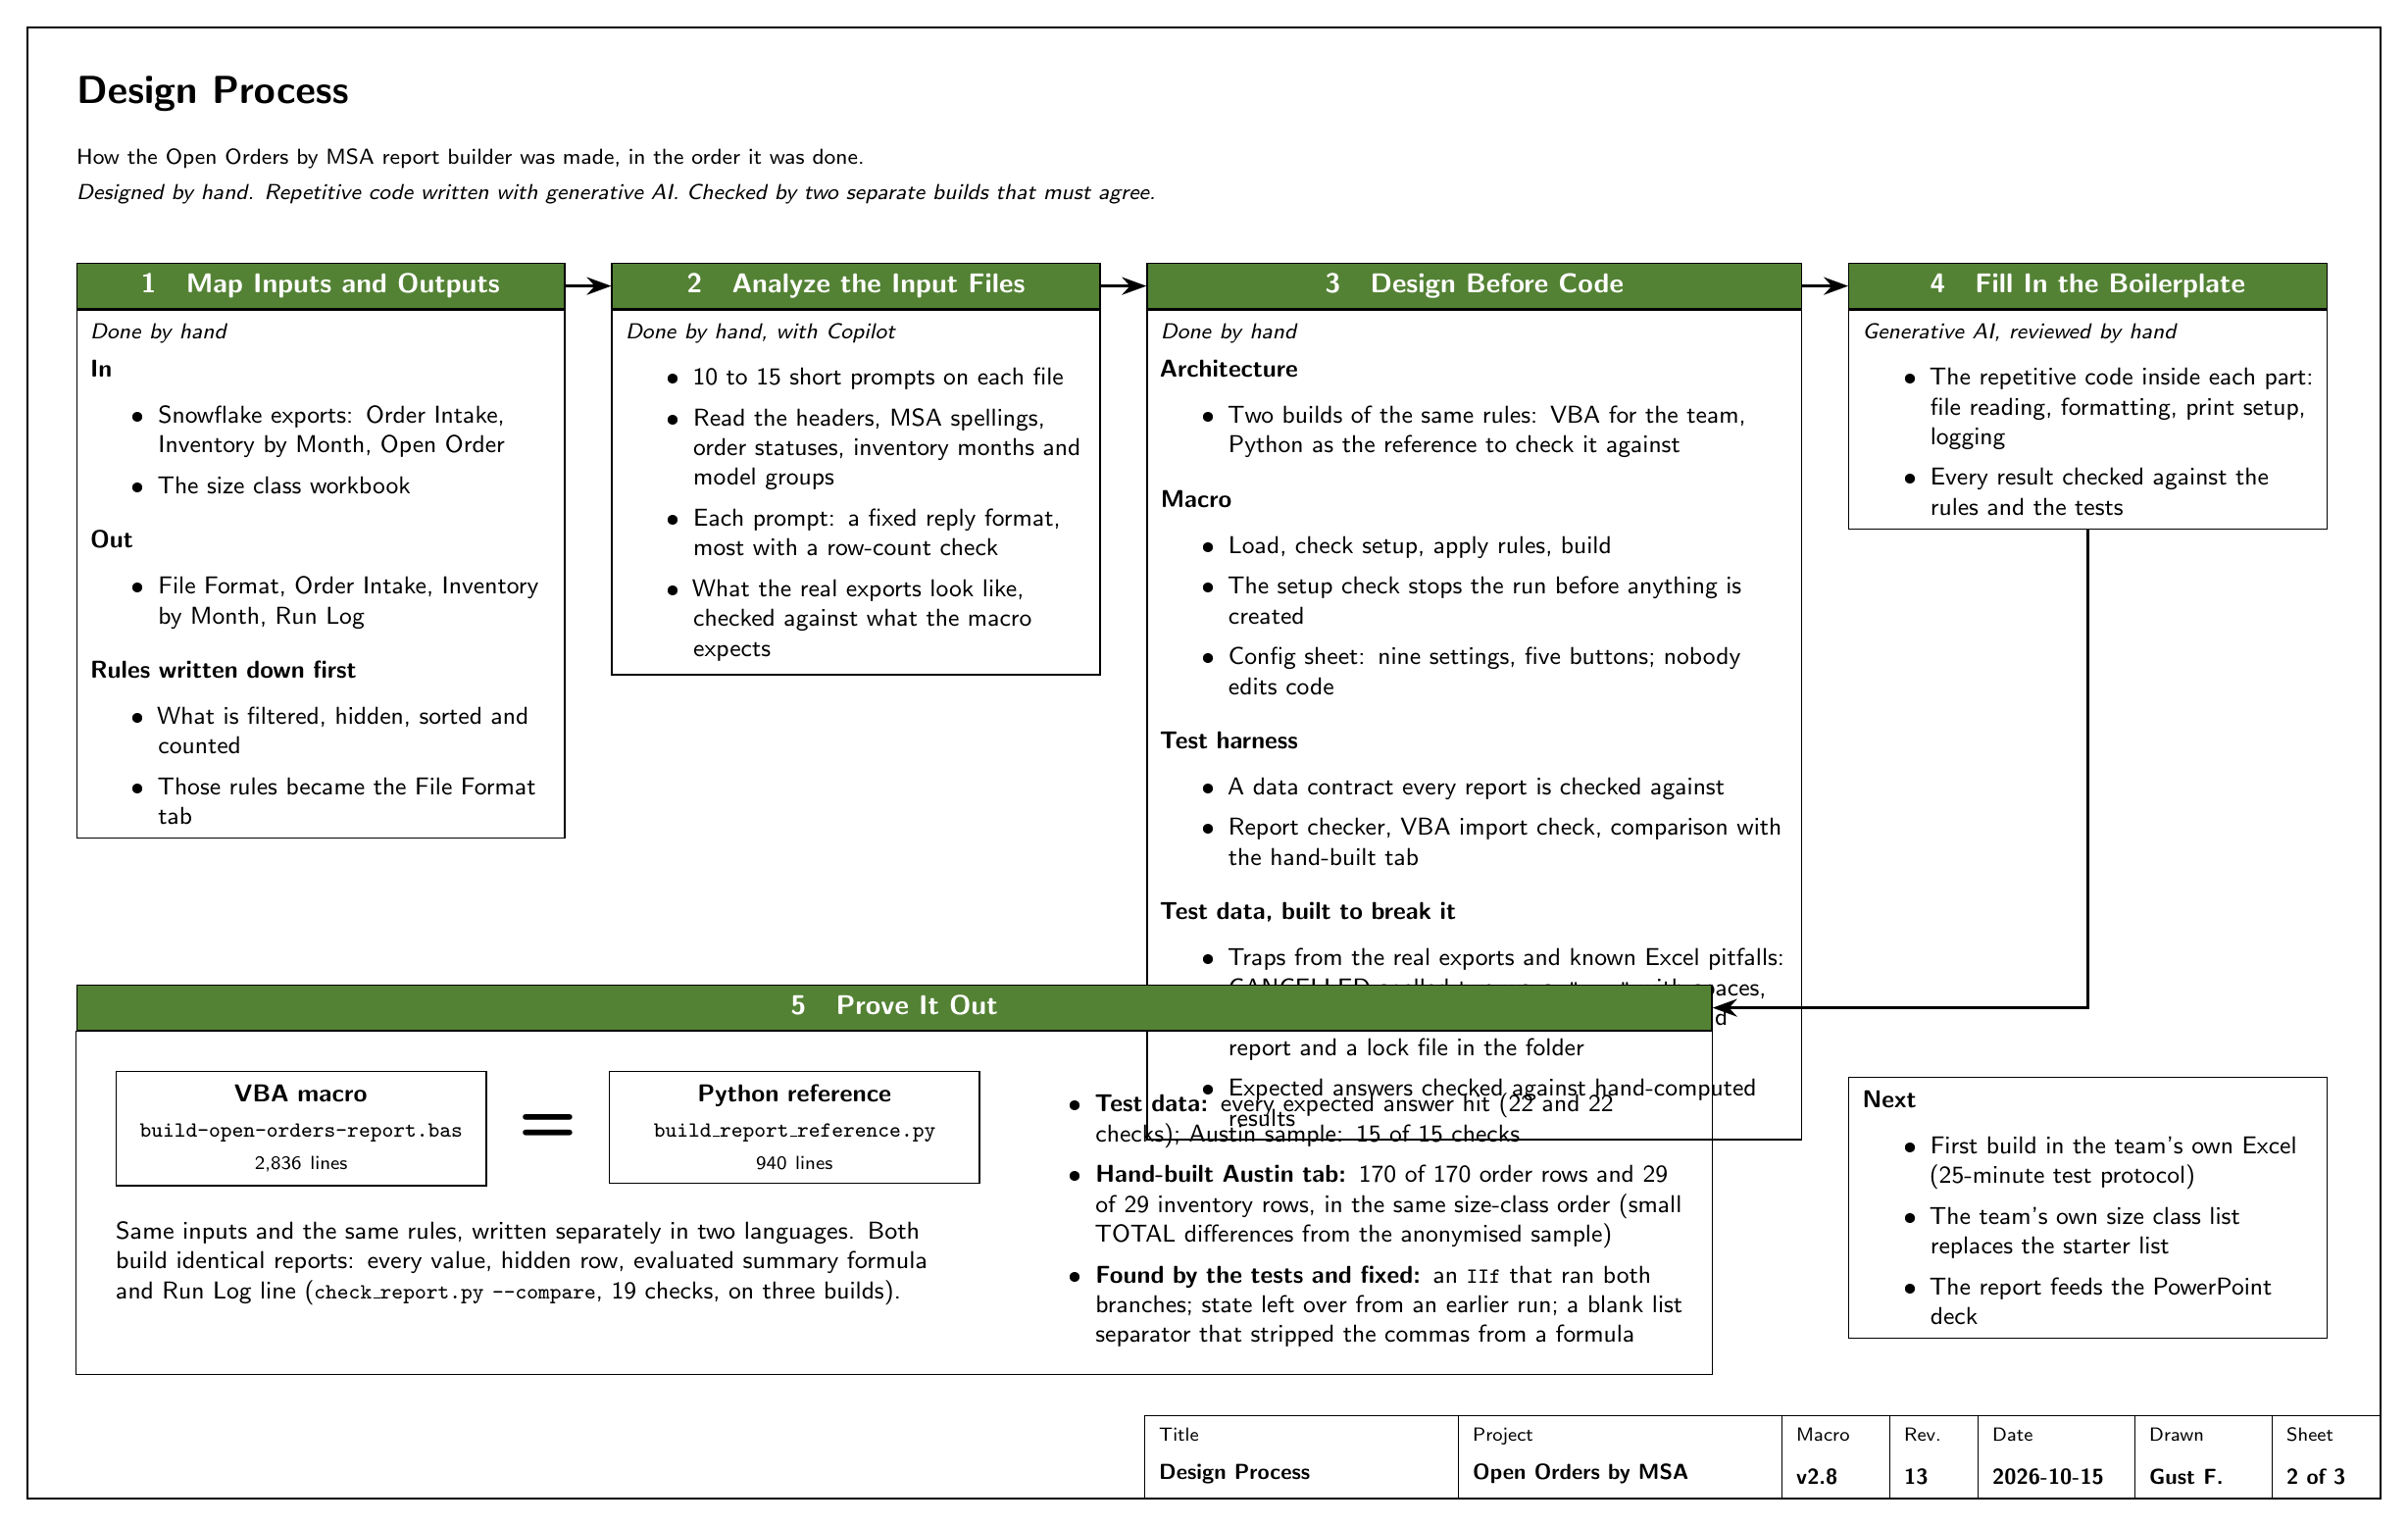
\begin{tikzpicture}[x=1in, y=1in]
\useasboundingbox (0,0) rectangle (12,7.5);
\draw[line width=0.8pt] (0,0) rectangle (12,7.5);

\node[anchor=north west, inner sep=0pt, font=\sffamily\bfseries\fontsize{14}{16}\selectfont]
  at (0.25,7.25) {Design Process};
\node[anchor=north west, inner sep=0pt, font=\sffamily\footnotesize] at (0.25,6.88)
  {How the Open Orders by MSA report builder was made, in the order it was done.};
\node[anchor=north west, inner sep=0pt, font=\sffamily\footnotesize\itshape] at (0.25,6.7)
  {Designed by hand. Repetitive code written with generative AI. Checked by two separate builds that must agree.};

% ---------------------------------------------------------------- step 1
\node[station, anchor=north west, text width=2.35in] (h1) at (0.25,6.3) {1\quad Map Inputs and Outputs};
\node[box, anchor=north, text width=2.35in] (b1) at (h1.south) {\by{Done by hand}
  \textbf{In}\\[1pt]
  \begin{itemize}
  \item Snowflake exports: Order Intake, Inventory by Month, Open Order
  \item The size class workbook
  \end{itemize}\vspace{3pt}
  \textbf{Out}\\[1pt]
  \begin{itemize}
  \item File Format, Order Intake, Inventory by Month, Run Log
  \end{itemize}\vspace{3pt}
  \textbf{Rules written down first}\\[1pt]
  \begin{itemize}
  \item What is filtered, hidden, sorted and counted
  \item Those rules became the File Format tab
  \end{itemize}};

% ---------------------------------------------------------------- step 2
\node[station, anchor=north west, text width=2.35in] (h2) at (2.979,6.3) {2\quad Analyze the Input Files};
\node[box, anchor=north, text width=2.35in] (b2) at (h2.south) {\by{Done by hand, with Copilot}
  \begin{itemize}
  \item 10 to 15 short prompts on each file
  \item Read the headers, MSA spellings, order statuses, inventory months and model groups
  \item Each prompt: a fixed reply format, most with a row-count check
  \item What the real exports look like, checked against what the macro expects
  \end{itemize}};

% ---------------------------------------------------------------- step 3
\node[station, anchor=north west, text width=3.2in] (h3) at (5.708,6.3) {3\quad Design Before Code};
\node[box, anchor=north, text width=3.2in] (b3) at (h3.south) {\by{Done by hand}
  \textbf{Architecture}\\[1pt]
  \begin{itemize}
  \item Two builds of the same rules: VBA for the team, Python as the reference to check it against
  \end{itemize}\vspace{3pt}
  \textbf{Macro}\\[1pt]
  \begin{itemize}
  \item Load, check setup, apply rules, build
  \item The setup check stops the run before anything is created
  \item Config sheet: nine settings, five buttons; nobody edits code
  \end{itemize}\vspace{3pt}
  \textbf{Test harness}\\[1pt]
  \begin{itemize}
  \item A data contract every report is checked against
  \item Report checker, VBA import check, comparison with the hand-built tab
  \end{itemize}\vspace{3pt}
  \textbf{Test data, built to break it}\\[1pt]
  \begin{itemize}
  \item Traps from the real exports and known Excel pitfalls: CANCELLED spelled two ways, {\footnotesize\texttt{" mx "}} with spaces,
        dates stored as text, an unknown model, an old report and a lock file in the folder
  \item Expected answers checked against hand-computed results
  \end{itemize}};

% ---------------------------------------------------------------- step 4
\node[station, anchor=north west, text width=2.3in] (h4) at (9.287,6.3) {4\quad Fill In the Boilerplate};
\node[box, anchor=north, text width=2.3in] (b4) at (h4.south) {\by{Generative AI, reviewed by hand}
  \begin{itemize}
  \item The repetitive code inside each part: file reading, formatting, print setup, logging
  \item Every result checked against the rules and the tests
  \end{itemize}};

\draw[flow] (h1.east) -- (h2.west);
\draw[flow] (h2.east) -- (h3.west);
\draw[flow] (h3.east) -- (h4.west);

% ---------------------------------------------------------------- step 5: prove it, the widest box
\node[station, anchor=north west, text width=8.2in] (h5) at (0.25,2.62) {5\quad Prove It Out};
\coordinate (b5sw) at ($(h5.south west)+(0,-1.75)$);
\draw[line width=0.5pt] (h5.south west) rectangle (b5sw -| h5.south east);
\draw[flow] (b4.south) |- (h5.east);

% the two builds and the equals sign
\node[box, anchor=north west, text width=1.75in, align=center] (vba) at ($(h5.south west)+(0.2,-0.2)$)
  {\textbf{VBA macro}\\[2pt] {\footnotesize\texttt{build-open-orders-report.bas}}\\[1pt] \lines{2,836}};
\node[box, anchor=north west, text width=1.75in, align=center] (py) at ($(vba.north east)+(0.62,0)$)
  {\textbf{Python reference}\\[2pt] {\footnotesize\texttt{build\_report\_reference.py}}\\[1pt] \lines{940}};
\node[font=\sffamily\bfseries\fontsize{30}{30}\selectfont, inner sep=0pt] at ($(vba.east)!0.5!(py.west)$) {=};
\node[anchor=north west, align=left, text width=4.3in, inner sep=0pt] at ($(vba.south west)+(0,-0.18)$)
  {Same inputs and the same rules, written separately in two languages. Both build identical reports:
  every value, hidden row, evaluated summary formula and Run Log line
  ({\footnotesize\texttt{check\_report.py --compare}}, 19 checks, on three builds).};

% the other evidence
\node[anchor=north west, align=left, text width=3.4in, inner sep=0pt] at ($(h5.south west)+(4.85,-0.2)$)
  {\begin{itemize}
  \item \textbf{Test data:} every expected answer hit (22 and 22 checks); Austin sample: 15 of 15 checks
  \item \textbf{Hand-built Austin tab:} 170 of 170 order rows and 29 of 29 inventory rows, in the same
        size-class order (small TOTAL differences from the anonymised sample)
  \item \textbf{Found by the tests and fixed:} an {\footnotesize\texttt{IIf}} that ran both branches; state
        left over from an earlier run; a blank list separator that stripped the commas from a formula
  \end{itemize}};

% ---------------------------------------------------------------- next, under step 4
\node[box, anchor=north west, text width=2.3in] (nx) at (9.287,2.15) {\textbf{Next}\\[2pt]
  \begin{itemize}
  \item First build in the team's own Excel (25-minute test protocol)
  \item The team's own size class list replaces the starter list
  \item The report feeds the PowerPoint deck
  \end{itemize}};

\titleblock{Design Process}{2 of 3}
\end{tikzpicture}}

\newpage
% ============================================================================ sheet 3: the build flow, from its own source
% Open Orders report macro v2.8: one build, from the exports to the workbook.
% One 11 x 17 landscape page (ledger, 17 x 11 in) drawn in TikZ, read top left to bottom right: title and what the macro does for every MSA,
% stations 1 to 5 with the setup-check gate and the UNMAPPED loop, the title block.
% Statements come from output/open-orders-intake-inventory/macro-flow-visual-implementation-plan.md, Section 5,
% as trimmed by the owner on 2026-10-13 (Rev. 2 to Rev. 12); Rev. 13 (2026-10-14) retitles it
% MSA Open Orders Reporting Macro -- User Manual and words the by-hand line as what the macro now does, for the person it is handed to.
% Rev. 14 (2026-10-14): fact-checked against the .bas; adds Before you start, the folder and size class choices, the
% size class rule, where the report is saved and what a warning means.
% Rev. 15 (2026-10-15, macro v2.7): the size class comes from the master list only; a model not on it is UNMAPPED.
% Rev. 16 (2026-10-15, macro v2.8): the allowed classes are on the master list's Set-up tab; a new class needs no code change.
% Laid out on a 12 x 7.5 in grid and scaled by 4/3 to fill the 16 x 10 in drawing area (type, lines and arrows scale with it).
% Build: ./build.sh source/open-orders-intake-inventory/open-orders-macro-flow.tex
\documentclass[10pt]{article}
\usepackage[paperwidth=17in, paperheight=11in, margin=0.5in]{geometry}
\usepackage[T1]{fontenc}
\usepackage{lmodern}
\usepackage{microtype}
\usepackage{enumitem}
\usepackage{xcolor}
\usepackage{tikz}
\usetikzlibrary{positioning, arrows.meta, calc, fit, shapes.geometric, intersections}
\usepackage[hidelinks, pdftitle={MSA Open Orders Reporting Macro - User Manual}, pdfauthor={Gust F.}]{hyperref}
\pagestyle{empty}
\setlength{\parindent}{0pt}
\hyphenpenalty=10000
\exhyphenpenalty=10000
\setlist[itemize]{label=\textbullet, leftmargin=0.85em, labelsep=0.35em, itemsep=1.5pt, parsep=0pt,
                  topsep=0pt, partopsep=0pt}
\definecolor{headgreen}{HTML}{548235}
\definecolor{flagpeach}{HTML}{FCE4D6}
% sheet number in the title block; open-orders-team-review.tex inputs this drawing (docmute) as one sheet of a set
\providecommand{\flowsheet}{1 of 1}
\tikzset{
  every node/.style={font=\sffamily\small, inner sep=5pt},
  box/.style={draw, line width=0.5pt, fill=white, align=left},
  station/.style={draw, line width=0.5pt, fill=headgreen, text=white, font=\sffamily\bfseries\normalsize,
                  align=center, inner ysep=4pt, text height=1.6ex, text depth=0.45ex},
  flow/.style={-{Stealth[length=9pt, width=6.5pt]}, line width=1.2pt, line join=miter},
  gate/.style={draw, line width=0.8pt, diamond, aspect=2, inner sep=4pt, font=\sffamily\bfseries\small},
  note/.style={font=\sffamily\footnotesize, inner sep=2pt},
  branch/.style={font=\sffamily\bfseries\small, inner sep=3pt},
  % flowchart document symbol: 1.55 x 0.42 in, wavy foot, anchored at its top left corner
  doc/.pic={\draw[line width=0.5pt, fill=white] (0,0) -- (1.55,0) -- (1.55,-0.36)
              .. controls (1.15,-0.5) and (0.45,-0.26) .. (0,-0.42) -- cycle;}
}

\begin{document}
\noindent
\scalebox{1.333333}{%
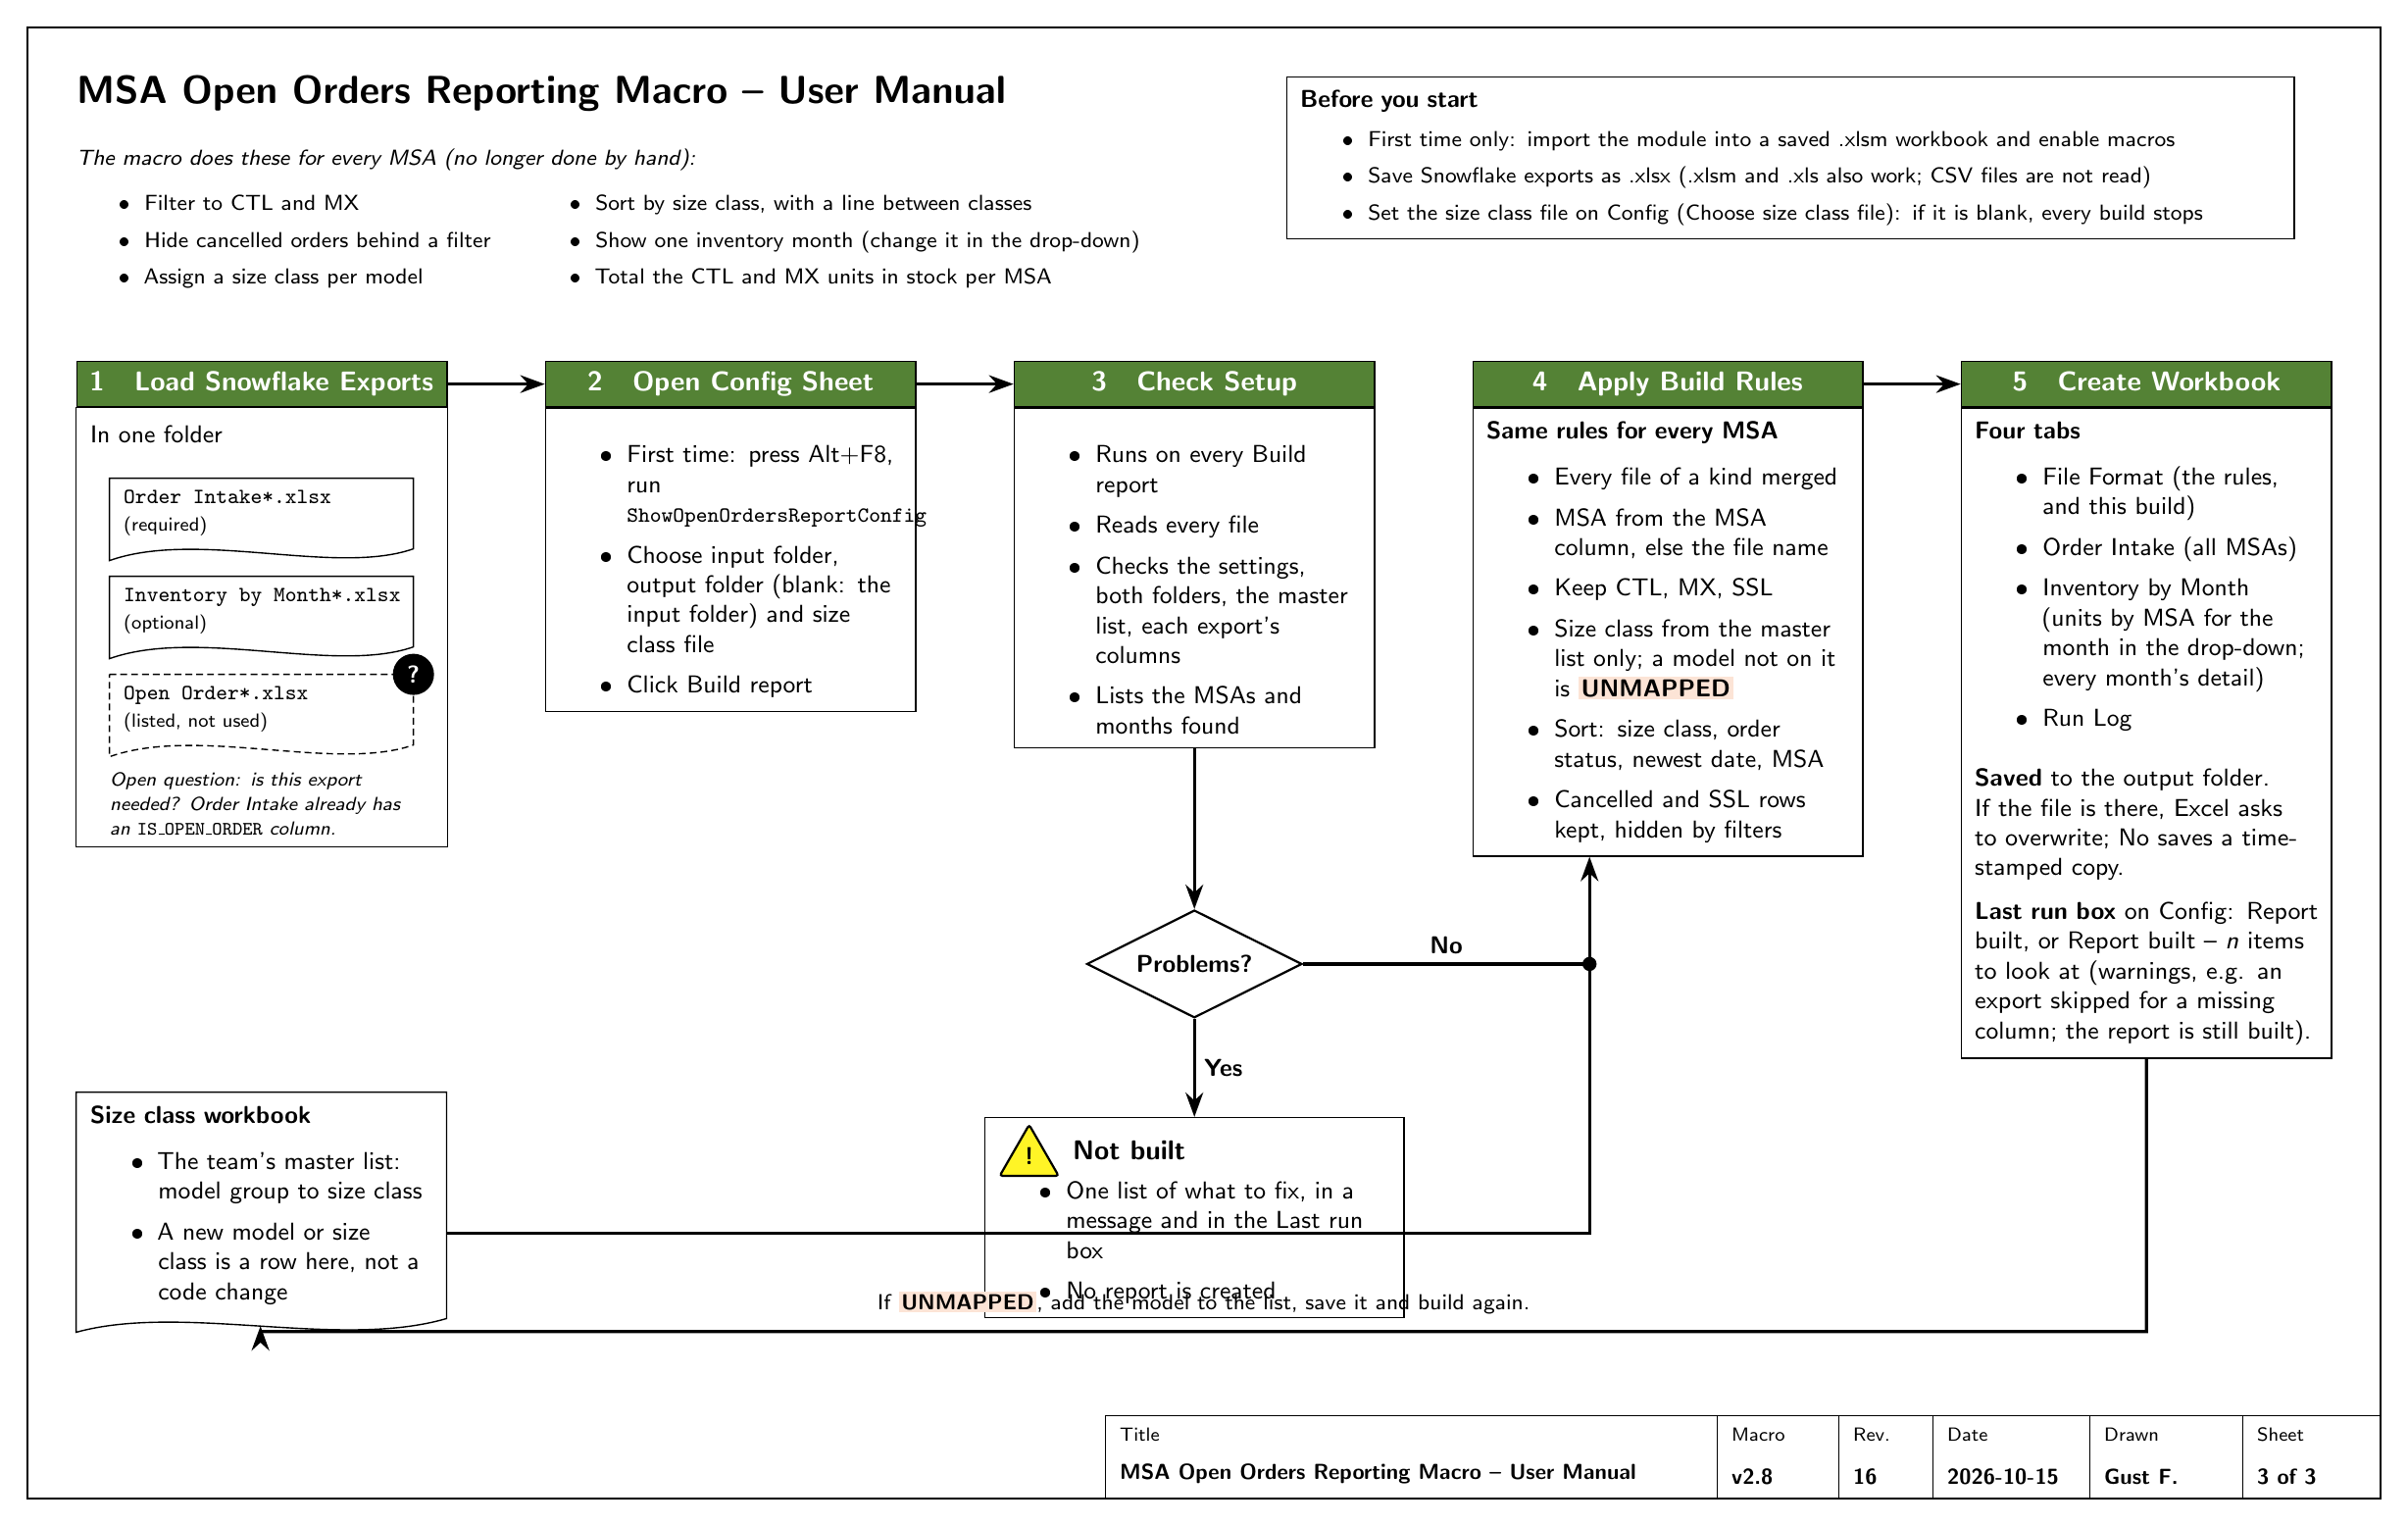
\begin{tikzpicture}[x=1in, y=1in]
\useasboundingbox (0,0) rectangle (12,7.5);

% ---------------------------------------------------------------- sheet frame
\draw[line width=0.8pt] (0,0) rectangle (12,7.5);

% ---------------------------------------------------------------- title and the by-hand line
\node[anchor=north west, inner sep=0pt, font=\sffamily\bfseries\fontsize{14}{16}\selectfont]
  at (0.25,7.25) {MSA Open Orders Reporting Macro -- User Manual};
\node[anchor=north west, inner sep=0pt, font=\sffamily\footnotesize\itshape] at (0.25,6.88) {The macro does these for every MSA (no longer done by hand):};
\node[anchor=north west, align=left, inner sep=0pt, text width=2.5in, font=\sffamily\footnotesize] at (0.25,6.74)
  {\begin{itemize}
  \item Filter to CTL and MX
  \item Hide cancelled orders behind a filter
  \item Assign a size class per model
  \end{itemize}};
\node[anchor=north west, align=left, inner sep=0pt, text width=3.3in, font=\sffamily\footnotesize] at (2.55,6.74)
  {\begin{itemize}
  \item Sort by size class, with a line between classes
  \item Show one inventory month (change it in the drop-down)
  \item Total the CTL and MX units in stock per MSA
  \end{itemize}};

% ---------------------------------------------------------------- before you start, top right
\node[box, anchor=north west, text width=5.0in, font=\sffamily\footnotesize] at (6.42,7.25) {\textbf{\small Before you start}\\[2pt]
  \begin{itemize}
  \item First time only: import the module into a saved .xlsm workbook and enable macros
  \item Save Snowflake exports as .xlsx (.xlsm and .xls also work; CSV files are not read)
  \item Set the size class file on Config (Choose size class file): if it is blank, every build stops
  \end{itemize}};

% ---------------------------------------------------------------- station 1: Snowflake exports, in one folder
\node[station, anchor=north west, text width=1.75in] (h1) at (0.25,5.8) {1\quad Load Snowflake Exports};
\draw[line width=0.5pt] (h1.south west) rectangle ($(h1.south east)+(0,-2.24)$);
\coordinate (b1) at ($(h1.south)+(0,-2.24)$);
\node[anchor=north west] at ($(h1.south west)+(0,-0.02)$) {In one folder};
\pic at ($(h1.south west)+(0.17,-0.36)$) {doc};
\node[anchor=north west, align=left, inner sep=0pt] at ($(h1.south west)+(0.24,-0.42)$)
  {{\footnotesize\texttt{Order Intake*.xlsx}}\\[-1pt]{\fontsize{7.5}{9}\selectfont(required)}};
\pic at ($(h1.south west)+(0.17,-0.86)$) {doc};
\node[anchor=north west, align=left, inner sep=0pt] at ($(h1.south west)+(0.24,-0.92)$)
  {{\footnotesize\texttt{Inventory by Month*.xlsx}}\\[-1pt]{\fontsize{7.5}{9}\selectfont(optional)}};
% the Open Order export: an open question, drawn dashed with a question mark and a one-line note
\pic[dash pattern=on 2.5pt off 1.5pt] at ($(h1.south west)+(0.17,-1.36)$) {doc};
\node[anchor=north west, align=left, inner sep=0pt] at ($(h1.south west)+(0.24,-1.42)$)
  {{\footnotesize\texttt{Open Order*.xlsx}}\\[-1pt]{\fontsize{7.5}{9}\selectfont(listed, not used)}};
\node[circle, fill=black, text=white, font=\sffamily\bfseries\small, inner sep=0pt, minimum size=0.21in]
  at ($(h1.south west)+(1.72,-1.36)$) {?};
\node[anchor=north west, align=left, inner sep=0pt, text width=1.6in, font=\sffamily\itshape\fontsize{7.5}{9}\selectfont]
  at ($(h1.south west)+(0.17,-1.86)$) {Open question: is this export needed? Order Intake already has an {\upshape\texttt{IS\_OPEN\_ORDER}} column.};

% ---------------------------------------------------------------- station 2: Config sheet
\node[station, anchor=north west, text width=1.75in] (h2) at (2.64,5.8) {2\quad Open Config Sheet};
\node[box, anchor=north, text width=1.75in] (b2) at (h2.south) {\begin{itemize}
  \item First time: press Alt+F8, run\\ {\footnotesize\texttt{ShowOpenOrdersReportConfig}}
  \item Choose input folder, output folder (blank: the input folder) and size class file
  \item Click Build report
  \end{itemize}};

% ---------------------------------------------------------------- station 3: setup check, the gate and the stop
\node[station, anchor=north west, text width=1.7in] (h3) at (5.03,5.8) {3\quad Check Setup};
\node[box, anchor=north, text width=1.7in] (b3) at (h3.south) {\begin{itemize}
  \item Runs on every Build report
  \item Reads every file
  \item Checks the settings, both folders, the master list, each export's columns
  \item Lists the MSAs and months found
  \end{itemize}};
\node[gate] (g) at ($(b3.south)+(0,-1.1)$) {Problems?};
\draw[flow] (b3.south) -- (g.north);
\node[box, anchor=north, text width=2.0in] (nb) at ($(g.south)+(0,-0.5)$) {{\normalsize\textbf{\phantom{Not built}}}\\[7pt]
  \begin{itemize}
  \item One list of what to fix, in a message and in the Last run box
  \item No report is created
  \end{itemize}};
\draw[flow] (g.south) -- (nb.north) node[midway, right, branch] {Yes};
% warning sign on the Not built box: the problem state (same sign as the manual's warning box)
\draw[line width=0.8pt, fill=yellow!85, rounded corners=1pt]
  ($(nb.north west)+(0.08,-0.3)$) -- ++(0.3,0) -- ++(-0.15,0.26) -- cycle;
\node[font=\sffamily\bfseries\small, inner sep=0pt] at ($(nb.north west)+(0.23,-0.2)$) {!};
\node[anchor=mid west, font=\sffamily\bfseries\normalsize, inner sep=0pt] at ($(nb.north west)+(0.45,-0.19)$) {Not built};

% ---------------------------------------------------------------- station 4: build
\node[station, anchor=north west, text width=1.85in] (h4) at (7.37,5.8) {4\quad Apply Build Rules};
\node[box, anchor=north, text width=1.85in] (b4) at (h4.south) {\textbf{Same rules for every MSA}\\[2pt]
  \begin{itemize}
  \item Every file of a kind merged
  \item MSA from the MSA column, else the file name
  \item Keep CTL, MX, SSL
  \item Size class from the master list only; a model not on it is {\setlength{\fboxsep}{1pt}\colorbox{flagpeach}{\textbf{UNMAPPED}}}
  \item Sort: size class, order status, newest date, MSA
  \item Cancelled and SSL rows kept, hidden by filters
  \end{itemize}};
% No: straight out of the gate until it joins the master-list line, which carries both up into Build
\coordinate (join) at ($(b4.south)+(-0.4,0)$);
\draw[line width=1.2pt] (g.east) -- (g.east -| join) node[pos=0.5, above, branch] {No};
\fill (g.east -| join) circle (2.6pt);

% ---------------------------------------------------------------- station 5: workbook
\node[station, anchor=north west, text width=1.75in] (h5) at (9.86,5.8) {5\quad Create Workbook};
\node[box, anchor=north, text width=1.75in] (b5) at (h5.south) {\textbf{Four tabs}\\[2pt]
  \begin{itemize}
  \item File Format (the rules, and this build)
  \item Order Intake (all MSAs)
  \item Inventory by Month (units by MSA for the month in the drop-down; every month's detail)
  \item Run Log
  \end{itemize}\vspace{5pt}
  \textbf{Saved} to the output folder. If the file is there, Excel asks to overwrite; No saves a time-stamped copy.\\[5pt]
  \textbf{Last run box} on Config: Report built, or Report built -- \textit{n} items to look at (warnings, e.g. an export skipped for a missing column; the report is still built).};

% ---------------------------------------------------------------- flow arrows along the header line
\draw[flow] (h1.east) -- (h2.west);
\draw[flow] (h2.east) -- (h3.west);
\draw[flow] (h4.east) -- (h5.west);

% ---------------------------------------------------------------- size class workbook, a document under station 1
\node[anchor=north west, align=left, text width=1.7in] (t6) at (0.25,2.07) {\textbf{Size class workbook}\\[2pt]
  \begin{itemize}
  \item The team's master list: model group to size class
  \item A new model or size class is a row here, not a code change
  \end{itemize}};
\draw[name path=scdoc, line width=0.5pt] (0.25,2.07) -- (2.139,2.07) -- (2.139,2.07 |- t6.south)
  .. controls ($(t6.south)+(0.42,-0.16)$) and ($(t6.south)+(-0.38,0.08)$) .. ($(0.25,0)+(0,0 |- t6.south)+(0,-0.07)$)
  -- cycle;

% master list into station 4: straight out of the document, one corner, up into Build
\draw[flow] (2.139,1.35) -| (join);

% return: UNMAPPED back to the master list, two right angles, ending on the document's wavy foot
\path[name path=up] (1.19,0) -- (1.19,2.07);
\path[name intersections={of=up and scdoc, sort by=up, by={foot}}];
\draw[flow] (b5.south) |- (1.19,0.85) -- (foot);
\node[anchor=south, note] at (6.0,0.91) {If {\setlength{\fboxsep}{1pt}\colorbox{flagpeach}{\textbf{UNMAPPED}}}, add the model to the list, save it and build again.};

% ---------------------------------------------------------------- title block, one row in the corner
\draw[line width=0.5pt] (5.5,0) -- (5.5,0.42) -- (12,0.42);
\foreach \x in {8.62, 9.24, 9.72, 10.52, 11.3} \draw[line width=0.5pt] (\x,0) -- (\x,0.42);
\foreach \x/\label/\value in {5.5/Title/MSA Open Orders Reporting Macro -- User Manual, 8.62/Macro/v2.8, 9.24/Rev./16,
                              9.72/Date/2026-10-15, 10.52/Drawn/Gust F., 11.3/Sheet/\flowsheet} {
  \node[anchor=north west, inner sep=0pt, font=\sffamily\fontsize{7}{8}\selectfont] at (\x+0.07,0.36) {\label};
  \node[anchor=south west, inner sep=0pt, font=\sffamily\bfseries\footnotesize] at (\x+0.07,0.07) {\value};
}

\end{tikzpicture}}
\end{document}
%
\end{document}
